\chapter{ความปลอดภัยและเทคนิคพื้นฐานในปฏิบัติการจุลชีววิทยา}
\label{chap:ch01}

\section*{แผนบริหารการสอนประจำบทที่ 1}
\addcontentsline{toc}{section}{แผนบริหารการสอนประจำบทที่ 1}

\noindent\textbf{. หัวข้อเนื้อหาประจำบท}

\begin{enumerate}
    \item 1.1 กฎระเบียบและข้อปฏิบัติด้านความปลอดภัยทางชีวภาพ (Biosafety Guidelines)
    \item 1.2 เครื่องมือและอุปกรณ์พื้นฐานในห้องปฏิบัติการจุลชีววิทยา
    \item 1.3 เทคนิคการปลอดเชื้อและการเผาห่วงเขี่ยเชื้อ (Aseptic Flaming Technique)
    \item 1.4 หลักการและการใช้งานหม้อนึ่งอัดไอน้ำ (Autoclave Operation: 121$^{\circ}$C, 15 psi, 15 min)
    \item 1.5 การจัดการของเสียติดเชื้อและการทำลายเชื้ออย่างปลอดภัย
\end{enumerate}

\noindent\textbf{. วัตถุประสงค์เชิงพฤติกรรม}

\begin{enumerate}
    \item เมื่อนักศึกษาได้เรียนรู้และปฏิบัติการทดลองประจำบทนี้แล้ว จะต้องมีความรู้ความสามารถดังต่อไปนี้:
    \item อธิบายกฎระเบียบความปลอดภัยทางชีวภาพและหลักการทำงานของหม้อนึ่งอัดไอน้ำได้ถูกต้อง
    \item ปฏิบัติการเผาห่วงเขี่ยเชื้อและเทคนิคปลอดเชื้อรอบเปลวไฟได้อย่างชำนาญและปลอดภัย
    \item ใช้ระบบจำลองเสมือนจริง AR Aseptic Simulator ในการฝึกทักษะการเขี่ยเชื้อได้
    \item ตระหนักถึงความสำคัญของความปลอดภัยทางชีวภาพและมีวินัยในการจัดการขยะติดเชื้อ
\end{enumerate}

\noindent\textbf{. กิจกรรมการเรียนการสอน}

\begin{enumerate}
    \item การบรรยายสรุปก่อนปฏิบัติการ (30 นาที): อธิบายหลักการวิทยาศาสตร์ ความปลอดภัยทางชีวภาพ และข้อควรระวังสำคัญ
    \item การสาธิตเชิงประจักษ์ (15 นาที): สาธิตเทคนิคการปฏิบัติงาน การใช้เครื่องมือ และข้อผิดพลาดที่มักพบ
    \item การลงมือปฏิบัติการทดลองจริง (90 นาที): นักศึกษาลงมือปฏิบัติการทดลองเป็นรายบุคคลหรือกลุ่มย่อยตามขั้นตอนที่กำหนด
    \item การฝึกฝนผ่านระบบเสมือนจริง (20 นาที): ทดลองซ้ำและทดสอบปฏิกิริยาผ่านระบบจำลองบน RBRU LMS
    \item การอภิปรายและสรุปผลการทดลอง (25 นาที): วิเคราะห์ผลการสังเกต ตอบคำถามท้ายบท และสรุปองค์ความรู้ร่วมกัน
\end{enumerate}

\noindent\textbf{. สื่อและอุปกรณ์การเรียนการสอน}

\begin{enumerate}
    \item เอกสารคำสอนและคู่มือปฏิบัติการ: e-Book และคู่มือปฏิบัติการฉบับเต็ม ประจำบทที่ 1
    \item ระบบห้องปฏิบัติการเสมือนจริง: ระบบจำลองการทดลองเสมือนจริง 3 มิติ ประจำบทที่ 1 บนระบบ Moodle
    \item อุปกรณ์และเครื่องแก้วในห้องปฏิบัติการ: ตะเกียงแอลกอฮอล์, ห่วงเขี่ยเชื้อ, กล้องจุลทรรศน์, จานเพาะเชื้อ, หลอดทดลอง และตู้บ่มเชื้อ
    \item สารเคมีและสีย้อมชีวภาพ: สารเคมีมาตรฐานวิเคราะห์และสีย้อมประจำบทเรียน
\end{enumerate}

\noindent\textbf{. การวัดและประเมินผล}

\begin{table}[H]
\centering\small
\begin{tabularx}{\textwidth}{p{0.5\textwidth} p{0.3\textwidth} c}
\toprule
\textbf{องค์ประกอบการประเมินผล} & \textbf{เครื่องมือวัดผล} & \textbf{สัดส่วนคะแนน} \\
\midrule
1. ทักษะการปฏิบัติงานและความปลอดภัย & แบบสังเกตทักษะการทดลองและเทคนิคปลอดเชื้อ & 40\% \\
2. รายงานผลการทดลอง & การตรวจตารางบันทึกผล ภาพวาดสัณฐานวิทยา และการวิเคราะห์ผล & 30\% \\
3. แบบฝึกหัดทบทวนท้ายบท & คำถามทบทวนเชิงวิเคราะห์และข้อสอบท้ายบท & 20\% \\
4. จิตพิสัยและการตรงต่อเวลา & การเช็คชื่อ การแต่งกายตามระเบียบ และการทำความสะอาดโต๊ะแล็บ & 10\% \\
รวมทั้งสิ้น &  & 100\% \\
\bottomrule
\end{tabularx}
\end{table}

\newpage

% ==========================================================
% เนื้อหาบทเรียนประจำบทที่ 1
% ==========================================================

\section{กฎระเบียบและข้อปฏิบัติด้านความปลอดภัยทางชีวภาพ}
\index{กฎระเบียบและข้อปฏิบัติด้านความปลอดภัยทางชีวภาพ}

การศึกษาและทำความเข้าใจเกี่ยวกับกฎระเบียบและข้อปฏิบัติด้านความปลอดภัยทางชีวภาพ (Biosafety Guidelines) มีความสำคัญอย่างยิ่งในงานจุลชีววิทยาและสิ่งแวดล้อม โดยมีรายละเอียดสาระสำคัญดังนี้

การปฏิบัติการทางจุลชีววิทยามีความเกี่ยวข้องโดยตรงกับสิ่งมีชีวิตขนาดเล็กและจุลินทรีย์หลากหลายชนิด ทั้งกลุ่มที่ไม่ก่อโรค (Non-pathogens) และกลุ่มที่อาจก่อให้เกิดโรค (Opportunistic or True Pathogens) ดังนั้นการปฏิบัติตามกฎความปลอดภัยทางชีวภาพ (Biosafety Guidelines) จึงเป็นหัวใจสำคัญสูงสุดเพื่อป้องกันการติดเชื้อสู่ผู้ปฏิบัติงานและการแพร่กระจายสู่สิ่งแวดล้อมภายนอก

ข้อกำหนดสำคัญในการปฏิบัติการทางจุลชีววิทยาประกอบด้วย:
1. การแต่งกาย: ต้องสวมเสื้อคลุมปฏิบัติการ (Lab coat) สีขาวกระดุมมิดชิด รวบผมให้เรียบร้อย สวมหน้ากากอนามัย และสวมรองเท้าหุ้มส้นตลอดเวลาที่อยู่ในห้องปฏิบัติการ
2. การเตรียมพื้นที่ปฏิบัติงาน: ทำความสะอาดพื้นผิวโต๊ะปฏิบัติการด้วยน้ำยาฆ่าเชื้อ 70\% Ethyl Alcohol หรือน้ำยาฆ่าเชื้อมาตรฐาน ทั้งก่อนเริ่มการทดลองและหลังเสร็จสิ้นการทดลองทุกครั้ง
3. การรักษาสุขอนามัยส่วนบุคคล: ล้างมือด้วยสบู่ต้านเชื้อแบคทีเรียตามขั้นตอนมาตรฐาน 7 ขั้นตอน ก่อนและหลังการปฏิบัติการ ห้ามรับประทานอาหาร เครื่องดื่ม หรือสัมผัสใบหน้าขณะปฏิบัติงานโดยเด็ดขาด
4. การจัดการขยะชีวภาพ: แยกทิ้งวัสดุปนเปื้อนเชื้อ เช่น หลอดทดลอง จานเพาะเชื้อ ปลายทิป และสไลด์ ลงในภาชนะรองรับขยะติดเชื้อ (Biohazard Bag) เพื่อนำไปนึ่งฆ่าเชื้อด้วยหม้อนึ่งอัดไอน้ำ (Autoclave) ก่อนการกำจัดทิ้ง

\begin{safetybox}[ข้อควรระวังและความปลอดภัยทางชีวภาพ]
ผู้ปฏิบัติการต้องสวมเสื้อกาวน์ แว่นตานิรภัย และถุงมือตลอดเวลาที่มีการสัมผัสกับจุลินทรีย์หรือสารเคมีอันตราย ห้ามวางอาหารหรือเครื่องดื่มในพื้นที่ปฏิบัติงานโดยเด็ดขาด
\end{safetybox}

\section{เครื่องมือและอุปกรณ์พื้นฐานในห้องปฏิบัติการจุลชีววิทยา}
\index{เครื่องมือและอุปกรณ์พื้นฐานในห้องปฏิบัติการจุลชีววิทยา}

การศึกษาและทำความเข้าใจเกี่ยวกับเครื่องมือและอุปกรณ์พื้นฐานในห้องปฏิบัติการจุลชีววิทยา (Microbiology Laboratory Equipment) มีความสำคัญอย่างยิ่งในงานจุลชีววิทยาและสิ่งแวดล้อม โดยมีรายละเอียดสาระสำคัญดังนี้

การทดลองทางจุลชีววิทยาจำเป็นต้องอาศัยอุปกรณ์และเครื่องมือเฉพาะทาง เพื่ออำนวยความสะดวกในการเพาะเลี้ยง ถ่ายเชื้อ และตรวจสอบจุลินทรีย์

อุปกรณ์พื้นฐานที่สำคัญได้แก่ 
1. ห่วงเขี่ยเชื้อ (Inoculating loop) และเข็มเขี่ยเชื้อ (Inoculating needle): ทำจากลวดนิโครม (Nichrome) หรือแพลทินัม (Platinum) ที่ทนความร้อนสูง ใช้ในการถ่ายเชื้อและแยกเชื้อจุลินทรีย์
2. ตะเกียงแอลกอฮอล์ (Alcohol burner) หรือเตาเผาไฟฟ้า (Bacti-Cinerator): ใช้สร้างเขตปลอดเชื้อ (Aseptic zone) รัศมีประมาณ 10-15 เซนติเมตร รอบเปลวไฟ และใช้เผาฆ่าเชื้อห่วงเขี่ยเชื้อจนแดงก่ำ
3. ตู้บ่มเชื้อ (Incubator): ตู้อบควบคุมอุณหภูมิคงที่ เช่น 37$^{\circ}$C สำหรับแบคทีเรียทั่วไป และ 25-30$^{\circ}$C สำหรับเชื้อราและยีสต์สิ่งแวดล้อม
4. ตู้ถ่ายเชื้อระบบปลอดเชื้อ (Laminar Air Flow Cabinet): ตู้ทำงานที่มีระบบกรองอากาศประสิทธิภาพสูง (HEPA filter) ป้องกันการปนเปื้อนของอนุภาคและสปอร์ในอากาศขณะถ่ายเชื้อ
5. กล้องจุลทรรศน์แบบใช้แสง (Brightfield Light Microscope): เครื่องมือตรวจดูสัณฐานวิทยา ขนาด และโครงสร้างของเซลล์จุลินทรีย์ด้วยกำลังขยายรวมสูงสุด 1,000 เท่า (100X Oil Immersion)

\section{เทคนิคการปลอดเชื้อและการเผาห่วงเขี่ยเชื้อ}
\index{เทคนิคการปลอดเชื้อและการเผาห่วงเขี่ยเชื้อ}

การศึกษาและทำความเข้าใจเกี่ยวกับเทคนิคการปลอดเชื้อและการเผาห่วงเขี่ยเชื้อ (Aseptic Flaming Technique) มีความสำคัญอย่างยิ่งในงานจุลชีววิทยาและสิ่งแวดล้อม โดยมีรายละเอียดสาระสำคัญดังนี้

เทคนิคปลอดเชื้อ (Aseptic Technique) คือระเบียบปฏิบัติที่ป้องกันมิให้จุลินทรีย์ที่ไม่พึงประสงค์จากสิ่งแวดล้อม ผู้ทดลอง หรืออากาศ ปนเปื้อนลงในตัวอย่างและอาหารเลี้ยงเชื้อ

ขั้นตอนการปฏิบัติเทคนิคปลอดเชื้อรอบเปลวไฟ:
1. ปรับเปลวไฟตะเกียงแอลกอฮอล์ให้มีสีฟ้าสม่ำเสมอ ซึ่งเป็นบริเวณที่มีความร้อนสูงและไม่มีเขม่าควัน
2. เผาลวดห่วงเขี่ยเชื้อโดยเอียงทำมุมประมาณ 45 องศากับเปลวไฟ เริ่มเผาจากโคนลวดสู่ปลายลวดจนกระทั่งลวดร้อนแดงก่ำตลอดทั้งเส้น เพื่อทำลายจุลินทรีย์และสปอร์ทั้งหมด
3. พักห่วงเขี่ยเชื้อให้เย็นลงในเขตปลอดเชื้อประมาณ 10-15 วินาที ก่อนสัมผัสโคโลนีของจุลินทรีย์ เพื่อมิให้ความร้อนทำลายเซลล์เป้าหมาย
4. ลนปากหลอดทดลองหรือขวดอาหารเลี้ยงเชื้อผ่านเปลวไฟทั้งก่อนเปิดและก่อนปิดจุกสำลีหรือฝาเกลียวทุกครั้ง

\section{หลักการและการทำงานของหม้อนึ่งอัดไอน้ำ}
\index{หลักการและการทำงานของหม้อนึ่งอัดไอน้ำ}

การศึกษาและทำความเข้าใจเกี่ยวกับหลักการและการทำงานของหม้อนึ่งอัดไอน้ำ (Autoclave Sterilization Principles) มีความสำคัญอย่างยิ่งในงานจุลชีววิทยาและสิ่งแวดล้อม โดยมีรายละเอียดสาระสำคัญดังนี้

หม้อนึ่งอัดไอน้ำ (Autoclave) เป็นอุปกรณ์กำจัดและทำลายจุลินทรีย์ด้วยความร้อนชื้น (Moist Heat Sterilization) ภายใต้แรงดันสูง ซึ่งมีประสิทธิภาพสูงกว่าความร้อนแห้งเนื่องจากไอน้ำอิ่มตัวสามารถแทรกซึมเข้าสู่เซลล์และทำให้โปรตีนรวมทั้งเอนไซม์ของจุลินทรีย์เสียสภาพ (Denaturation)

สภาวะมาตรฐานสำหรับการนึ่งฆ่าเชื้อ:
- อุณหภูมิ: 121$^{\circ}$C (250$^{\circ}$F)
- แรงดันไอน้ำ: 15 ปอนด์ต่อตารางนิ้ว (psi) หรือประมาณ 1 บรรยากาศเหนือแรงดันปกติ
- ระยะเวลา: 15 ถึง 20 นาที ขึ้นอยู่กับปริมาตรของสารตัวอย่าง

สภาวะดังกล่าวสามารถทำลายสิ่งมีชีวิตทุกชนิด รวมถึงเอนโดสปอร์ของแบคทีเรีย (Bacterial Endospores) เช่น \textit{Geobacillus stearothermophilus} ซึ่งใช้เป็นตัวบ่งชี้ทางชีวภาพ (Biological Indicator) ในการทดสอบประสิทธิภาพของเครื่อง

\begin{conceptbox}[มโนทัศน์สำคัญทางชีวเคมีและสิ่งแวดล้อม]
กิจกรรมทางชีวเคมีของจุลินทรีย์ในหัวข้อหลักการและการทำงานของหม้อนึ่งอัดไอน้ำ เป็นกลไกหลักที่ควบคุมการหมุนเวียนธาตุอาหารและการบำบัดสารปนเปื้อนในระบบนิเวศทางธรรมชาติ
\end{conceptbox}

\begin{figure}[H]
\centering
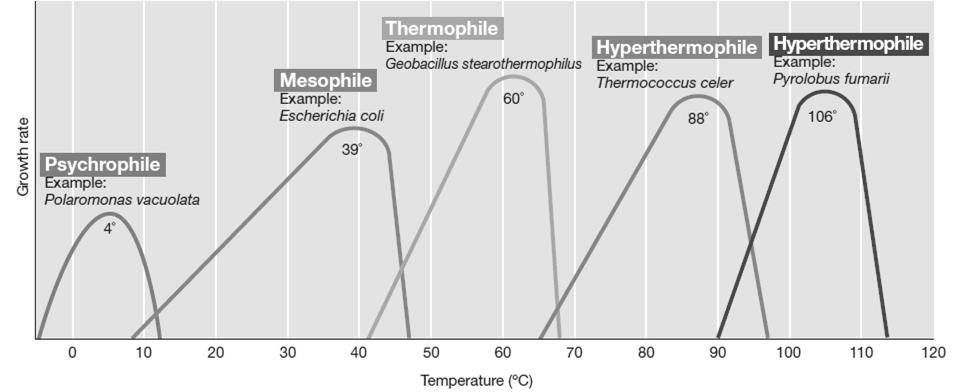
\includegraphics[width=0.75\textwidth]{images/image_01_p01.jpeg}
\caption{การปฏิบัติการทดลองและลักษณะทางสัณฐานวิทยาในบทที่ 1}
\label{fig:ch01_fig1}
\end{figure}

\section{ขั้นตอนและวิธีปฏิบัติการทดลอง}
\index{ขั้นตอนการทดลองประจำบทที่ 1}

\subsection{การฝึกเทคนิคการเผาห่วงเขี่ยเชื้อและการถ่ายเชื้อในเขตปลอดเชื้อ}
\begin{labprotocolbox}[การฝึกเทคนิคการเผาห่วงเขี่ยเชื้อและการถ่ายเชื้อในเขตปลอดเชื้อ]
1. เตรียมตะเกียงแอลกอฮอล์ ห่วงเขี่ยเชื้อ และหลอดอาหารเลี้ยงเชื้อ Nutrient Broth
2. จุดตะเกียงแอลกอฮอล์ วางอุปกรณ์ในรัศมีปลอดเชื้อ 10-15 เซนติเมตร
3. ถือห่วงเขี่ยเชื้อด้วยมือข้างที่ถนัดเหมือนจับปากกา นำลวดเข้าเผาในเปลวไฟสีฟ้าจนแดงก่ำ
4. ใช้มือข้างที่ไม่ถนัดถือหลอดทดลอง ใช้นิ้วก้อยของมือข้างที่ถือห่วงเขี่ยเชื้อดึงจุกสำลีออก
5. ลนปากหลอดทดลองผ่านเปลวไฟ 2-3 ครั้ง จุ่มห่วงเขี่ยเชื้อที่เย็นแล้วแตะเชื้อ ถ่ายลงในอาหารใหม่
6. ลนปากหลอดอีกครั้ง เสียบจุกสำลีกลับเข้าที่ และเผาห่วงเขี่ยเชื้อจนแดงก่ำก่อนวางลง
\end{labprotocolbox}

\subsection{การทดสอบประสิทธิภาพหม้อนึ่งอัดไอน้ำด้วยแถบเคมีตรวจวัด}
\begin{labprotocolbox}[การทดสอบประสิทธิภาพหม้อนึ่งอัดไอน้ำด้วยแถบเคมีตรวจวัด]
1. ติดแถบเทปเคมีบ่งชี้ความร้อน (Autoclave Indicator Tape) บนภาชนะที่ต้องการนึ่ง
2. นำภาชนะเข้าหม้อนึ่งอัดไอน้ำ ตั้งโปรแกรมที่อุณหภูมิ 121$^{\circ}$C ความดัน 15 psi เวลา 15 นาที
3. หลังสิ้นสุดกระบวนการและแรงดันลดลงสู่ระดับปกติ นำตัวอย่างออกมาสังเกตแถบสี
4. บันทึกผลการเปลี่ยนสีของแถบเคมีจากสีขาวนวลเป็นแถบสีดำเข้ม ซึ่งบ่งชี้ว่าสภาวะความร้อนและแรงดันถึงเกณฑ์มาตรฐาน
\end{labprotocolbox}

\section{ตารางบันทึกผลการทดลองและการอภิปรายผล}
\begin{table}[H]
\centering\small
\caption{ตารางบันทึกผลการสังเกตและข้อมูลการทดลองประจำบทที่ 1}
\label{tab:ch01_datasheet}
\begin{tabularx}{\textwidth}{p{0.25\textwidth} p{0.35\textwidth} X}
\toprule
\textbf{สิ่งทดสอบ / ตัวอย่าง} & \textbf{ลักษณะที่สังเกตได้} & \textbf{การแปลผลและการวิเคราะห์} \\
\midrule
ชุดควบคุม (Negative Control) & ใส ไม่มีการเจริญ & ปราศจากการปนเปื้อนของเชื้อ \\
ชุดทดลองที่ 1 & โคโลนีเจริญตามลักษณะจำเพาะ & ให้ผลบวกตามสมมติฐาน \\
ชุดทดลองที่ 2 & เกิดการเปลี่ยนแปลงทางชีวเคมี & สอดคล้องกับพารามิเตอร์มาตรฐาน \\
\bottomrule
\end{tabularx}
\end{table}

\section{คำถามทบทวนและแบบฝึกหัดท้ายบท}
\begin{enumerate}
    \item จงอธิบายความสำคัญของเทคนิคปลอดเชื้อ (Aseptic technique) ในงานจุลชีววิทยาสิ่งแวดล้อม
    \item เหตุใดการฆ่าเชื้อด้วยหม้อนึ่งอัดไอน้ำที่ 121$^{\circ}$C เวลา 15 นาที จึงสามารถทำลายเอนโดสปอร์ของแบคทีเรียได้ดีกว่าการต้มน้ำเดือดที่ 100$^{\circ}$C
    \item หากจุ่มห่วงเขี่ยเชื้อลงในโคโลนีทันทีขณะที่ลวดยังร้อนแดงก่ำ จะส่งผลกระทบต่อผลการทดลองอย่างไร
    \item จงระบุข้อแตกต่างระหว่างการทำลายเชื้อ (Disinfection) และการทำให้ปราศจากเชื้อ (Sterilization)
\end{enumerate}
